\documentclass[conference]{IEEEtran}
\IEEEoverridecommandlockouts
% The preceding line is only needed to identify funding in the first footnote. If that is unneeded, please comment it out.
\usepackage{cite}
\usepackage{amsmath,amssym
b,amsfonts}
\usepackage{algorithmic}
\usepackage{graphicx}
\usepackage{textcomp}
\usepackage{xcolor}
\usepackage{siunitx}
\def\BibTeX{{\rm B\kern-.05em{\sc i\kern-.025em b}\kern-.08em
T\kern-.1667em\lower.7ex\hbox{E}\kern-.125emX}}
\begin{document}

\title{Energy-Efficient Communication in UAV-assisted Batteryless Wireless Sensor Networks}

\author{
  \IEEEauthorblockN{Miguel Brandt}
  \IEEEauthorblockA{\textit{Department of Informatics} \\
    \textit{Pontifical Catholic University of Rio de Janeiro} \\
    Rio de Janeiro, Brazil \\
  miguelperes@aluno.puc-rio.br}
  \and
  \IEEEauthorblockN{Kelvin Bittencourt}
  \IEEEauthorblockA{\textit{Department of Electrical Engineering} \\
    \textit{Pontifical Catholic University of Rio de Janeiro} \\
    Rio de Janeiro, Brazil \\
  kelvinbitt@gmail.com}
  \and
  \IEEEauthorblockN{Adriano Branco}
  \IEEEauthorblockA{\textit{Department of Informatics} \\
    \textit{Pontifical Catholic University of Rio de Janeiro} \\
    Rio de Janeiro, Brazil \\
  abranco@inf.puc-rio.br}
  \and
  \IEEEauthorblockN{Markus Endler}
  \IEEEauthorblockA{\textit{Department of Informatics} \\
    \textit{Pontifical Catholic University of Rio de Janeiro} \\
    Rio de Janeiro, Brazil \\
  endler@inf.puc-rio.br}
}

\maketitle

\begin{abstract}
  A number of studies have been proposed to tackle the task of monitoring large areas by deploying a wireless sensor network. When communication infrastructure is unavailable, or the region is not easily accessible, data can be retrieved from such networks by using Unmanned Aerial Vehicles (UAVs) as gateways to a base station, thus creating a UAV-assisted Wireless Sensor Network (UAV-WSN).

  However, providing regular maintenance for an extensive, scattered WSN is impractical, leading to devices with limited service life, usually tied to their battery lifespan. Further, they are often treated as disposable, and as a result, become chemical waste.

  In this ongoing study, we explore the integration of batteryless sensors powered by energy harvesting (EH) within UAV-WSNs. Since energy-efficient sensors cannot be continuously powered on, we begin by investigating techniques for establishing communication between sensors in a sleep state and UAVs, and ultimately focus on passive wake-up radios, proposing a simple design and discussing the results of real-world experiments.
\end{abstract}

\section{Introduction}

Mobile data sink nodes have been increasingly used to support wireless sensor networks in remote or hard-to-reach areas(CITE GRADYS). In UAV-WSNs, UAVs act as dynamic gateways, enabling data transfer from localized sensors to a base station, which then relays data to the cloud for further processing. This approach can be valuable for applications such as environmental monitoring(CITE) and precision agriculture(CITE).

One of the challenges with WSNs in remote areas is the reliance on battery-powered sensors, which have limited lifespans and contribute to environmental waste (CITE). Energy harvesting offers a potential solution by enabling sensors to operate without batteries, instead drawing energy from ambient sources like solar or radiofrequency (RF) waves (CITE). However, EH systems pose difficulties of their own, including limited and fluctuating power availability, dependence on environmental conditions, and the need for efficient energy management(CITE). These limitations often result in intermittent operation, where sensors cannot be continuously active(CITE).

\section{Energy-Efficient Communication}

Traditional duty cycling is a common technique for reducing energy consumption in WSNs(CITE), by periodically switching sensors between active and sleep states. While this approach can extend battery life, it introduces latency and limits network responsiveness(CITE), as sensors are unavailable during sleep periods. Wake-up receiver (WuRx)-based solutions offer a more efficient alternative, as they allow sensors to remain in a deep sleep state until activated by an external signal, therefore drastically reducing energy use(CITE).

There are various WuRx options(CITE), including optical and acoustic receivers, each suited for specific applications. Optical receivers are often used in line-of-sight scenarios, such as indoor lighting systems(CITE), while acoustic receivers are common in underwater networks or areas where RF propagation is limited(CITE). However, wake-up radios (WuR) are particularly suitable for UAV-WSNs due to their ability to provide reliable, long-range activation without the need for line-of-sight(CITE). Figure \ref{fig:drone_over_sensor} shows one of our test scenarios, a UAV with a transmitter approaching a sensor powered by solar energy harvesting, connected to a prototype passive WuR.

TODO: justificar melhor ter escolhido wake-up radios, e as aplicacoes dos outros tipos. revisar esse segundo paragrafo em geral, primeiro ta ok.

falar que e porque escolhemos um passivo, e o que é passivo

mention addressing capabilities for targeted wake-up

\begin{figure}[htbp]
  \centerline{\includegraphics[width=0.8\linewidth]{drone_flying_over_sensor.jpg}}
  \caption{UAV approaching a batteryless sensor}
  \label{fig:drone_over_sensor}
\end{figure}

\section{Experiment and Results}

\subsection{Test Environment}

In order to conduct experiments, we assembled a passive wake-up radio on a protoboard using off-the-shelf components, based on a voltage doubler circuit, with a 17.3~cm quarter-wave monopole copper wire antenna, and a 50~$\Omega$ matching network, as we expect to receive a 433~MHz signal. Since the primary function of the WuR is to trigger an interrupt in the sensor's GPIO ports, we've also included a 1N4728A voltage clamping Zener diode of 3.3~V to prevent accidental overvoltage on the microcontroller. The circuit is depicted in Figure \ref{fig:receiver}.

\begin{figure}[htbp]
  \centerline{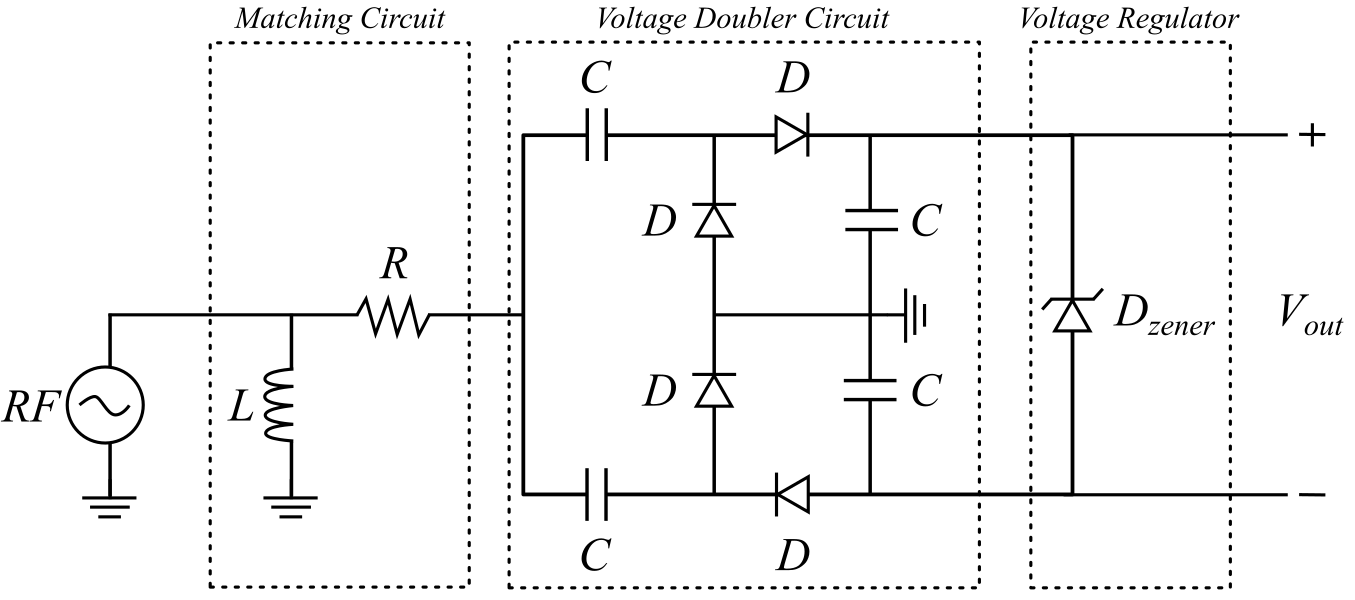
\includegraphics[width=1\linewidth]{receiver.png}}
  \caption{Passive wake-up radio schematic}
  \label{fig:receiver}
\end{figure}

In this instance, we performed in-lab measurements with the transmitter powered directly by a DC power supply. The transmitter is a CC1101 radio connected to an ESP32, which is programmed to continuously send a carrier wave with arbitrary data at its maximum power of +12~dBm, in the 433~MHz frequency range. The receiver is connected to an oscilloscope for measuring output voltage, as we hope to achieve at least 2.3~V, which is the minimum threshold for interrupt detection by low-power microcontrollers, namely our MSP430-equipped sensor node.

Although initial tests were performed indoors, we've also built an autonomous, programmable and modular UAV, as seen in Figure \ref{fig:drone_over_sensor}, in order to assess more realistic scenarios.

\subsection{Preliminary Findings}

Experiments revealed that the transmitter's output power was unable to charge the receiver's capacitors at a significant rate, except when their antennas were less than 1~cm apart, at which point we attribute the energy transfer to near-field coupling, rather than far-field RF harvesting. Because the UAV cannot hover on top of the receiver for too long, it is essential that the voltage rapidly reaches 2.3~V. Ideally, the UAV would fly over the sensor and collect the necessary data without any deceleration.

As a point of reference, we've also performed tests with a commercial 433~MHz handheld transceiver capable of 2-3~W (33-34.7~dBm) output power, which was able to quickly generate an interrupt on the receiver at a 30~cm distance while transmitting. With this observation, we believe that an active amplifier must be utilized, either on the transmitter, using the UAV's battery as a power source, or at the receiver output, borrowing power from the sensor's energy harvester. We plan to compare both solutions in our next phase of research.

\section{Conclusion}

The preliminary findings of this research highlight both the potential and challenges of employing passive wake-up radio receivers. While the in-lab tests confirmed that RF energy harvesting is feasible, achieving efficient energy transfer at practical distances remains unresolved. Additional development in the energy transmission and harvesting process is necessary to achieve the desired outcome. Further studies may focus on better antenna designs and circuit optimization for RF operation.

Moreover, the research will focus on conducting comprehensive outdoor tests with a fully equipped UAV to measure the impact of external variables such as motor and weather interference and communication reliability with a non stationary transmitter. By addressing these challenges, we hope to advance the practical implementation of sustainable, batteryless sensor networks within a UAV-WSN setting.

summarize findings

next steps

want to conduct outdoors tests with the drone, amplifier mounted, measure motor interference

optimize energy transfer: investigate better antenna designs, dipole antenna option ignores ground plane

% \bibliographystyle{IEEEtran}
% \bibliography{references}

\end{document}
